\chapter{Implementacija i korisničko sučelje}
		
		
		\section{Korištene tehnologije i alati}
		
			\textbf{\textit{dio 2. revizije}}
			
			 \noindent Za komunikaciju među članovima tima korišten je Whatsapp (https://www.whatsapp.com/), za raspodijelu zadataka među članovima tima korišten je Miro (https://miro.com/). Kao sustav za upravljanje izvornim kodom korišten je Git (https://git-scm.com/), a za udaljeni repozitorij projekta korišten je GitLab ( https://gitlab.com/). Za izradu UML dijagrama u dokumentaciji korišten je Astah UML (https://astah.net/).Za izradu backend dijela aplikacije korišten je programski jezik python (https://www.python.org/) verzija 3.8, te alat Flask (https://flask.palletsprojects.com/en/1.1.x/). Kao aplikacijski server korišten je heroku (https://heroku.com/).Korištena je baza podataka MySQL (https://www.mysql.com/).

			
			
			\eject 
		
	
		\section{Ispitivanje programskog rješenja}
			
			\textbf{\textit{dio 2. revizije}}\\
			
			 \textit{U ovom poglavlju je potrebno opisati provedbu ispitivanja implementiranih funkcionalnosti na razini komponenti i na razini cijelog sustava s prikazom odabranih ispitnih slučajeva. Studenti trebaju ispitati temeljnu funkcionalnost i rubne uvjete.}
	
			
			\subsection{Ispitivanje komponenti}
			
			\begin{figure}[H]
				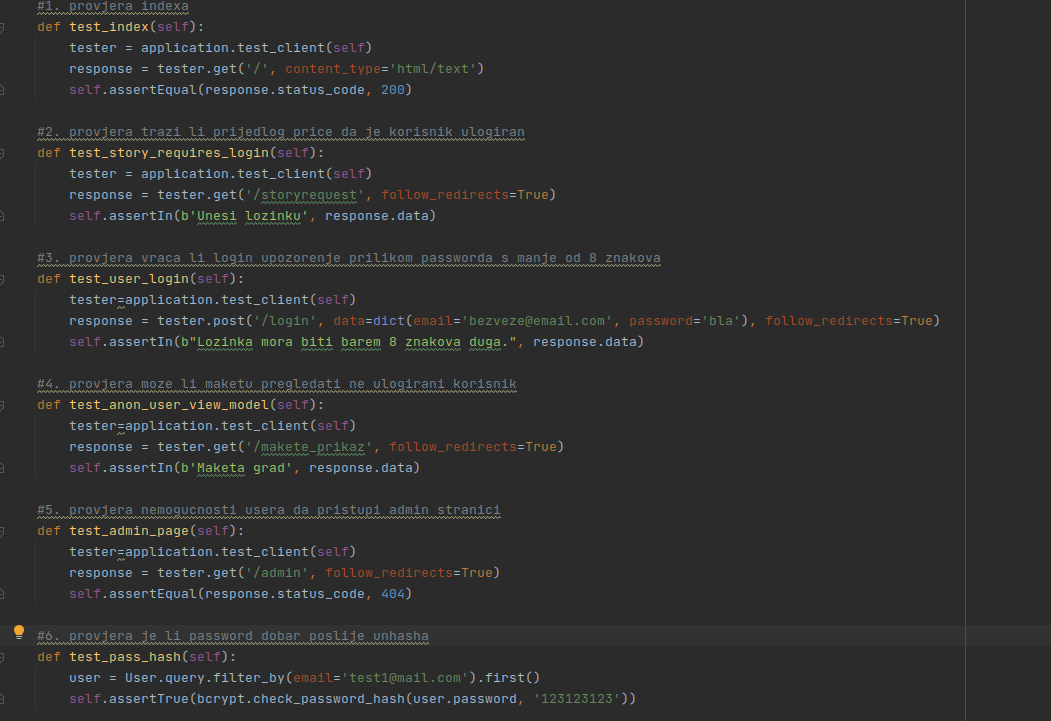
\includegraphics[width=1\linewidth]{slike/unit_tests.PNG} %veličina u odnosu na širinu linije
				\caption{Ispitivanje jedinica}
				\label{fig:unit1} %label mora biti drugaciji za svaku sliku
			\end{figure}
		
			\begin{figure}[H]
				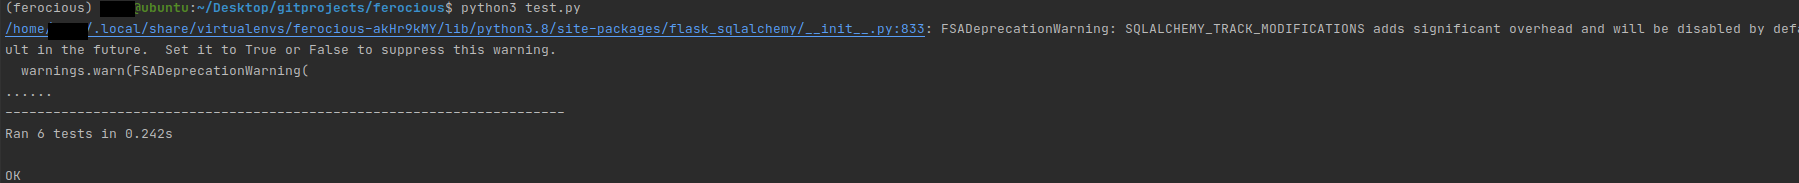
\includegraphics[width=1\linewidth]{slike/unit_test_result.PNG} %veličina u odnosu na širinu linije
				\caption{Rezultat ispitivanja jedinica}
				\label{fig:unit2} %label mora biti drugaciji za svaku sliku
			\end{figure}
			
			
			\subsection{Ispitivanje sustava}
			
			 \noindent Provedeno je testiranje rada sustava pomoću Selenium testova(Selenium IDE)
			 . Testirane su neke od osnovnih funkcionalnosti sustava. Svi testovi izvrseni su ručno. U dokumentaciji su prikazani slučajevi UC1, UC9, UC10, UC11, UC23.

			\noindent Ispitni slučaj 1 : Registracija

			\noindent Ulaz : 
	
			\begin{itemize}
				\item : 1. Otvaranje pocetne stranice u web pregledniku.
				\item   2. Odabir na gumb registracije
				\item   3. Unos potrebnih podataka
			\end{itemize}

			\noindent Ocekivani rezultat : 

			\begin{itemize}
				\item : 1.a Prikazao se ekran za unos podataka
				\item   1.b Ako su uneseni valjani podaci korisnik ce biti preusmjeren na login screen
			\end{itemize}
	
			\noindent Rezultati : Očekivani rezultat 1.b je zadovoljen. Aplikacija je prošla test. 

			\begin{figure}[H]
				\includegraphics[width=1\linewidth]{slike/ispitnit_test_1.PNG} %veličina u odnosu na širinu linije
				\caption{Ispitni test 1}
				\label{fig:Test1} %label mora biti drugaciji za svaku sliku
			\end{figure}
			
			\noindent Ispitni slučaj 2 : Prijava

			\noindent Ulaz : 
	
			\begin{itemize}
				\item : 1. Otvaranje pocetne stranice u web pregledniku.
				\item   2. Odabir na gumb prijava
				\item   3. Unos potrebnih podataka
			\end{itemize}

			\noindent Ocekivani rezultat : 

			\begin{itemize}
				\item : 1.a Prikazao se ekran za unos podataka
				\item   1.b Ako su uneseni valjani podaci korisnik ce biti preusmjeren na pocetnu stranicu
			\end{itemize}
	
			\noindent Rezultati : Očekivani rezultat 1.b je zadovoljen. Aplikacija je prošla test. 

			\begin{figure}[H]
				\includegraphics[width=1\linewidth]{slike/ispitnit_test_2.PNG} %veličina u odnosu na širinu linije
				\caption{Ispitni test 2}
				\label{fig:Test2} %label mora biti drugaciji za svaku sliku
			\end{figure}			

			\noindent Ispitni slučaj 3 : Odjava

			\noindent Ulaz : 
	
			\begin{itemize}
				\item : 1. Korisnik treba biti prijavljen
				\item   2. Odabir na gumb odjavi se
			\end{itemize}

			\noindent Ocekivani rezultat : 

			\begin{itemize}
				\item : 1. Korisnik će biti odjavljen i preusmjeren na pocetnu stranicu
			\end{itemize}
	
			\noindent Rezultati : Očekivani rezultat 1. je zadovoljen. Aplikacija je prošla test. 

			\begin{figure}[H]
				\includegraphics[width=1\linewidth]{slike/ispitnit_test_3.PNG} %veličina u odnosu na širinu linije
				\caption{Ispitni test 3}
				\label{fig:Test3} %label mora biti drugaciji za svaku sliku
			\end{figure}	

			\noindent Ispitni slučaj 4 : Odjava

			\noindent Ulaz : 
	
			\begin{itemize}
				\item : 1. Korisnik treba biti prijavljen
				\item   2. Odabir na gumb moj profil
			\end{itemize}

			\noindent Ocekivani rezultat : 

			\begin{itemize}
				\item : 1. Korisnik će biti preusmjeren na stranicu sa svojim podacima
			\end{itemize}
	
			\noindent Rezultati : Očekivani rezultat 1. je zadovoljen. Aplikacija je prošla test. 

			\begin{figure}[H]
				\includegraphics[width=1\linewidth]{slike/ispitnit_test_4.PNG} %veličina u odnosu na širinu linije
				\caption{Ispitni test 4}
				\label{fig:Test4} %label mora biti drugaciji za svaku sliku
			\end{figure}				

			\noindent Ispitni slučaj 5 : Postavljanje postavki vidljivosti korisničkog računa

			\noindent Ulaz : 
	
			\begin{itemize}
				\item : 1. Korisnik treba biti prijavljen
				\item   2. Odabir na gumb uredi
				\item   3. Odabir postavki vidljivosti
				\item   4. Pritisak na gumb spremi promjene
			\end{itemize}

			\noindent Ocekivani rezultat : 

			\begin{itemize}
				\item : 1.a Korisnik će biti preusmjeren na stranicu postavka profila
				\item   1.b Nakon odabira postavka privatnosti i pristika na gumb korisnik će biti preusmjeren na stranicu sa svojim podacima.
			\end{itemize}
	
			\noindent Rezultati : Očekivani rezultat 1.b je zadovoljen. Aplikacija je prošla test. 

			\begin{figure}[H]
				\includegraphics[width=1\linewidth]{slike/ispitnit_test_5.PNG} %veličina u odnosu na širinu linije
				\caption{Ispitni test 5}
				\label{fig:Test5} %label mora biti drugaciji za svaku sliku
			\end{figure}

			\eject 
		
		
		\section{Dijagram razmještaja}
			
			 Dijagram razmještaja je strukturni statički UML dijagram koji opisuje topologiju sustava i usredotočen je na odnos sklopovskih i programskih dijelova. Postoji više vrsta dijagrama razmještaja, a ovdje se koristi specifikacijski dijagram razmještaja kako bi se prije navedeni odnos prikazao. Za ostvarenje ove aplikacije se koristi arhitektura "klijent - poslužitelj", a komunikacija se odvija protokolom HTTP. Na klijentskoj strani se nalazi web preglednik pomoću kojeg korisnik pristupa poslužitelju, odnosno šalje HTTP zahtjeve i prima HTTP odgovore. Poslužiteljska strana je nešto složenija te se ona sastoji od web poslužitelja na koji pristižu HTTP zahtjevi i poslužitelja baze podataka kojem web poslužitelj pristupa i iz kojeg uzima, uređuje ili sprema podatke.
			 
			 \begin{figure}[H]
			 	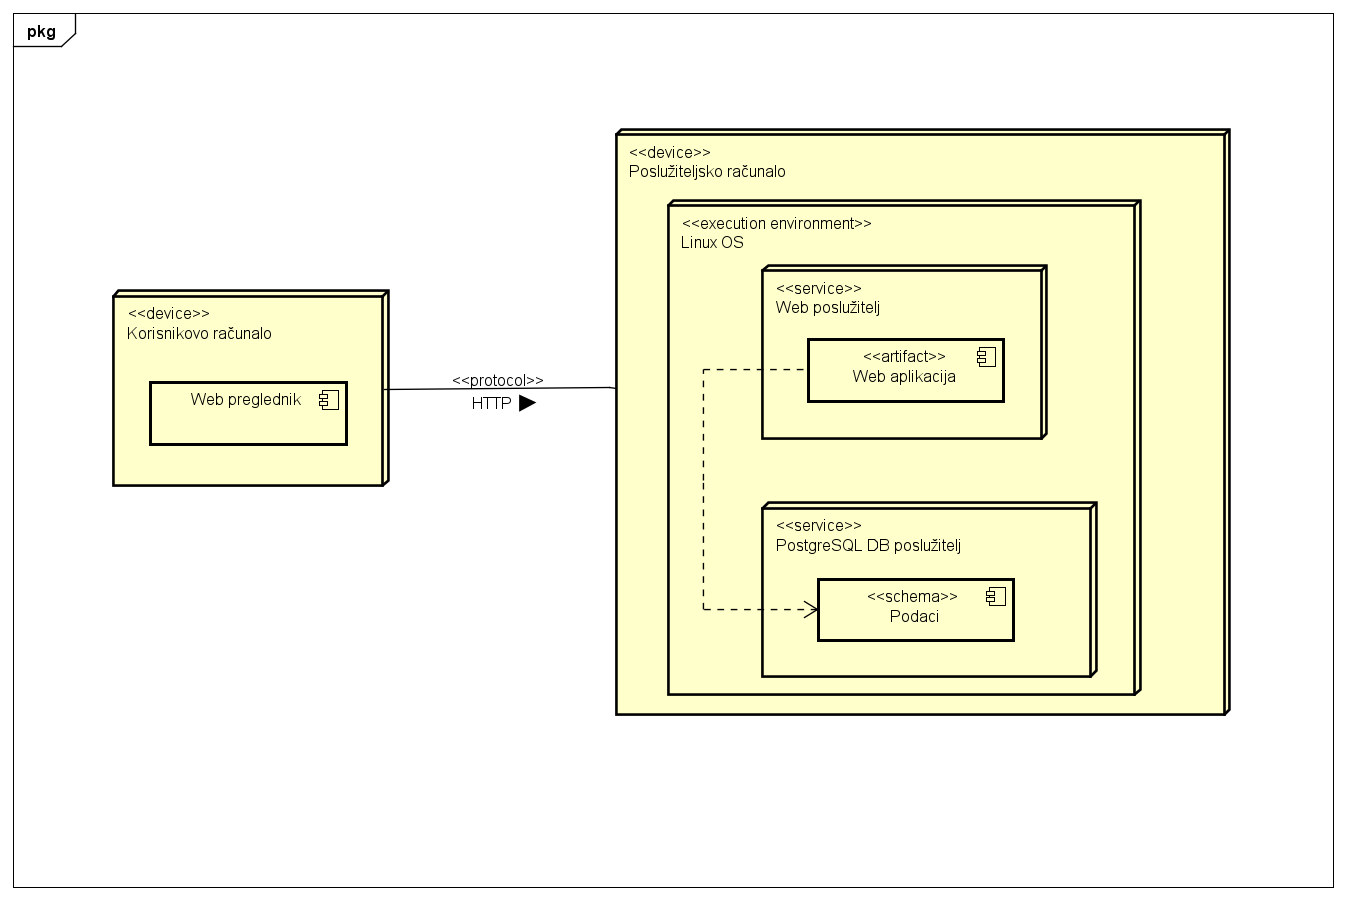
\includegraphics[width=1\linewidth]{slike/Dijagram_razmjestaja.PNG} %veličina u odnosu na širinu linije
			 	\caption{Dijagram razmještaja}
			 	\label{fig:dijraz} %label mora biti drugaciji za svaku sliku
			 \end{figure}
			
			\eject 
		
		\section{Upute za puštanje u pogon}
		
			\textbf{\textit{dio 2. revizije}}\\
		
			 \textit{U ovom poglavlju potrebno je dati upute za puštanje u pogon (engl. deployment) ostvarene aplikacije. Na primjer, za web aplikacije, opisati postupak kojim se od izvornog kôda dolazi do potpuno postavljene baze podataka i poslužitelja koji odgovara na upite korisnika. Za mobilnu aplikaciju, postupak kojim se aplikacija izgradi, te postavi na neku od trgovina. Za stolnu (engl. desktop) aplikaciju, postupak kojim se aplikacija instalira na računalo. Ukoliko mobilne i stolne aplikacije komuniciraju s poslužiteljem i/ili bazom podataka, opisati i postupak njihovog postavljanja. Pri izradi uputa preporučuje se \textbf{naglasiti korake instalacije uporabom natuknica} te koristiti što je više moguće \textbf{slike ekrana} (engl. screenshots) kako bi upute bile jasne i jednostavne za slijediti.}
			
			
			 \textit{Dovršenu aplikaciju potrebno je pokrenuti na javno dostupnom poslužitelju. Studentima se preporuča korištenje neke od sljedećih besplatnih usluga: \href{https://aws.amazon.com/}{Amazon AWS}, \href{https://azure.microsoft.com/en-us/}{Microsoft Azure} ili \href{https://www.heroku.com/}{Heroku}. Mobilne aplikacije trebaju biti objavljene na F-Droid, Google Play ili Amazon App trgovini.}
			
			
			\eject 